% figures/perceptual-map.tex
% Standalone TikZ: 2x2 perceptual map — price vs ease of implementation,
%   mid-market CRM category (ch.04 segmentation-targeting-positioning).
% Compiled to figures/perceptual-map.pdf via tools/build-figures.sh.
\documentclass[tikz,border=6pt]{standalone}
\usepackage{tikz}
\usetikzlibrary{arrows.meta,positioning,calc}

\definecolor{vcblue}{HTML}{1A5276}
\definecolor{vcteal}{HTML}{0E6655}
\definecolor{vcgray}{HTML}{4D4D4D}
\definecolor{vcred}{HTML}{922B21}
\definecolor{vcamber}{HTML}{7D6608}

\begin{document}
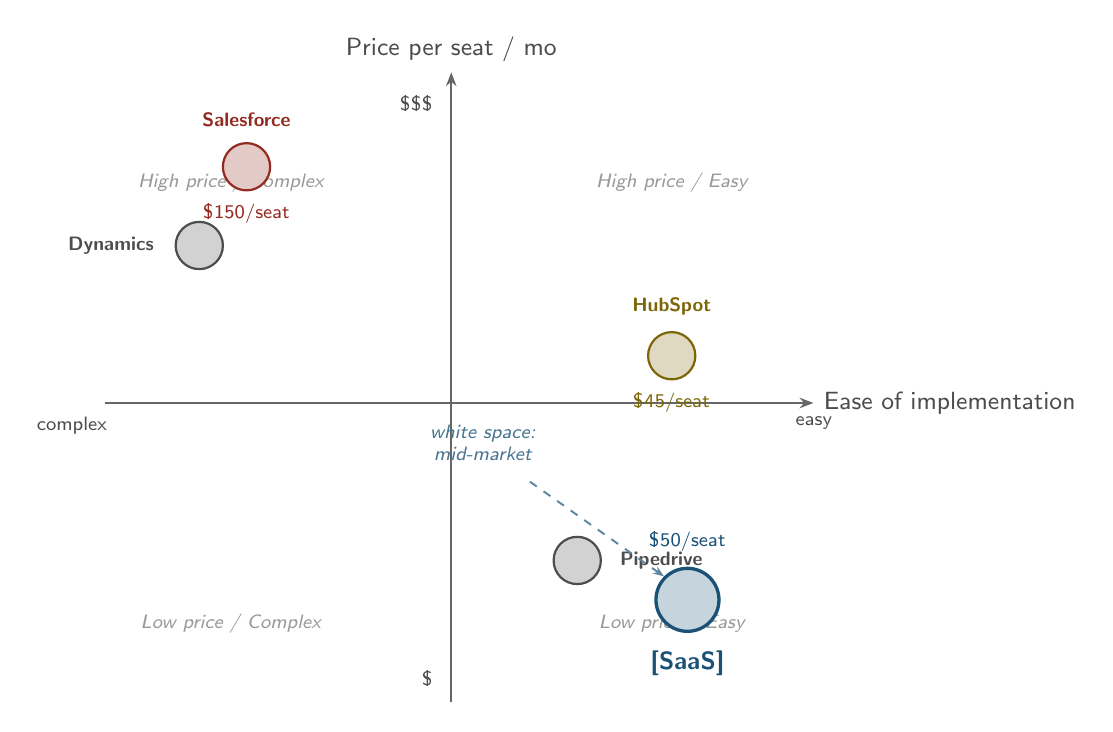
\begin{tikzpicture}[
  dot/.style={circle, draw=#1, fill=#1!25, line width=0.8pt,
              minimum size=6mm, font=\sffamily\scriptsize, text=black!85},
  axlbl/.style={font=\sffamily\small, text=black!70},
  quadlbl/.style={font=\sffamily\scriptsize\itshape, text=black!40},
]

%% ---- axes ----
% x-axis: Ease of Implementation (left=complex, right=easy)
% y-axis: Price per seat/month (bottom=low, top=high)
\draw[-{Stealth[length=5pt]}, line width=0.9pt, black!60]
  (-4.4,0) -- (4.6,0) node[right, axlbl] {Ease of implementation};
\draw[-{Stealth[length=5pt]}, line width=0.9pt, black!60]
  (0,-3.8) -- (0,4.2) node[above, axlbl] {Price per seat / mo};

%% ---- axis tick labels ----
\node[axlbl, below left=2pt] at (-4.2,0) {\scriptsize complex};
\node[axlbl, below right=2pt] at (4.2,0) {\scriptsize easy};
\node[axlbl, left=3pt] at (0,-3.5) {\scriptsize \$};
\node[axlbl, left=3pt] at (0,3.8) {\scriptsize \$\$\$};

%% ---- quadrant labels ----
\node[quadlbl] at (-2.8, 2.8) {High price / Complex};
\node[quadlbl] at ( 2.8, 2.8) {High price / Easy};
\node[quadlbl] at (-2.8,-2.8) {Low price / Complex};
\node[quadlbl] at ( 2.8,-2.8) {Low price / Easy};

%% ---- competitor dots ----
% Salesforce: high price, complex implementation
\node[dot=vcred] (sf) at (-2.6, 3.0)
  {\phantom{X}};
\node[font=\sffamily\scriptsize\bfseries, text=vcred, above=2pt of sf]
  {Salesforce};
\node[font=\sffamily\scriptsize, text=vcred, below=1pt of sf]
  {\$150/seat};

% HubSpot: moderate price, easy — SMB-first
\node[dot=vcamber] (hs) at (2.8, 0.6)
  {\phantom{X}};
\node[font=\sffamily\scriptsize\bfseries, text=vcamber, above=2pt of hs]
  {HubSpot};
\node[font=\sffamily\scriptsize, text=vcamber, below=1pt of hs]
  {\$45/seat};

% Microsoft Dynamics: high price, complex
\node[dot=vcgray] (dyn) at (-3.2, 2.0)
  {\phantom{X}};
\node[font=\sffamily\scriptsize\bfseries, text=vcgray, left=4pt of dyn]
  {Dynamics};

% Pipedrive: low price, moderate ease — SMB
\node[dot=vcgray] (pd) at (1.6, -2.0)
  {\phantom{X}};
\node[font=\sffamily\scriptsize\bfseries, text=vcgray, right=3pt of pd]
  {Pipedrive};

%% ---- our SaaS dot (highlighted) ----
\node[dot=vcblue, minimum size=8mm, line width=1.2pt] (us) at (3.0, -2.5)
  {\phantom{X}};
\node[font=\sffamily\small\bfseries, text=vcblue, below=3pt of us]
  {[SaaS]};
\node[font=\sffamily\scriptsize, text=vcblue, above=2pt of us]
  {\$50/seat};

%% ---- white-space annotation arrow ----
\draw[-{Stealth[length=4pt]}, vcblue!70, dashed, line width=0.7pt]
  (1.0,-1.0) -- (us.north west);
\node[font=\sffamily\scriptsize\itshape, text=vcblue!80, align=center]
  at (0.4,-0.5) {white space:\\mid-market};

\end{tikzpicture}
\end{document}
